\documentclass[pdftex,10pt]{article}
\usepackage{fullpage}
\usepackage{graphicx}
\usepackage{natbib}
\usepackage{amsmath}

\title{Storm surge modelling in the Strait of Georgia}
\author{Nancy Soontiens, Susan Allen, Doug Latornell, Kate Le Sou\"{e}f, Idalia Machuca}
\date{\today}

\begin{document}
\maketitle

\begin{abstract}
The Strait of Georgia is a large, semi-enclosed body of water between Vancouver Island and the mainland of British Columbia connected to the Pacific Ocean via the Strait of Juan de Fuca at the south and Johnstone Strait at the north. During the winter months, coastal communities in the Strait of Georgia are at risk to flooding caused by storm surges, a natural hazard that can occur when a strong storm coincides with high tide. This investigation produces storm surge hindcasts using a three-dimensional numerical ocean model for the Strait of Georgia and the surrounding bodies of water (Strait of Juan de Fuca, Puget Sound, and Johnstone Strait) collectively known as the Salish Sea. The numerical model employs the Nucleus for European Modelling of the Ocean (NEMO) architecture in a regional configuration. The model is evaluated through comparisons of tidal harmonics, tidal current ellipses, and storm surge water levels with observations. Important forcing factors contributing to storm surges have been assessed, finding that the surge entering the domain from the Pacific Ocean contributes most significantly. In addition, local wind patterns cause a slight increase in surge amplitude on the mainland side of the Strait of Georgia when compared to the Vancouver Island coastal areas. Surge amplitudes are found to be greater within the Strait of Georgia when compared to amplitudes in the Strait of Juan de Fuca. 
%needs a little more work.
\end{abstract}

\section{Introduction}\label{sec:intro}


%some general intro paragraph here. Need something about SoG size, geography, islands, sills, rivers, tides....
The Strait of Georgia is a strongly stratified, semi-enclosed body of water located between Vancouver Island and the mainland of British Columbia. It is part of a larger system of waterways collectively known as the Salish Sea and is connected to the Pacific Ocean via the Strait of Juan de Fuca and Johnstone Strait. It is on average 222 km in length and 28 km wide and its maximum depth is 420 m \citep{thomson1981oceanography}. At its southern end, the Strait of Georgia is connected to the Strait of Juan de Fuca through several passages, the largest being Haro Strait. The San Juan and Gulf Islands are scattered throughout these passages where complex bathymetry and steep topographic slopes induce vigorous tidal mixing. Many rivers feed fresh water into the Salish Sea system, the most significant source being from the Fraser River. Mixed diurnal and semi-diurnal tides are found throughout most of the Salish Sea but a semi-diurnal amphidrome is present nearby Victoria, where the tides are mainly diurnal. This system is home to several large coastal communities, such as Vancouver and Victoria, serves as a waterway for commercial traffic and recreational use, and supports a large and active fishing industry.   

%my attempt at physical oceanography in SoG- Susan feel free to edit.
Several features related to the physical oceanography of this region render it a challenge to model numerically. The outflow from the Fraser River in the late spring is the primary source fresh water within the Strait of Georgia and leads to large vertical density gradients in the summer months. Additionally, strong tidal mixing through the San Juan and Gulf Islands produces horizontal density gradients that separate the saline waters of the Strait of Juan de Fuca and the fresher water of the Strait of Georgia. It is important to accurately represent the vertical mixing in this region as it sets the rate of export of fresh water through estuarine circulation. The strong and fast tidal currents through the narrow channels of the north, such as Discovery Passage and Johnstone Strait, pose a particular challenge for numerical models. Yet, several modelling efforts for this region exist, ranging in choices of grid structure, mixing parametrizations, and domain size and extent. 

%overview oF SoG/Salish Sea models
Early work by \citet{crean1988mathematical,crean1988numerical} and \citet{stronach1993update} resulted in a series of models covering the Strait of Juan de Fuca, the Strait of Georgia and Puget Sound using a finite difference discretization of the equations of motion. A barotropic version of their model was used to reproduce storm surge water level elevations with reasonable accuracy, however, this barotropic version did not include the effects of fresh water entering the system from rivers. Later, a baroclinic version of their model examined residual circulation and fresh water flushing rates \citep{stronach1993update, marinone1996model}. This early work pointed to an important connection between the model's bottom friction parametrization and the location and amplitude of the M$_2$ amphidrome. They found that a local increase in the bottom friction coefficient, especially in the area of Haro Strait, was necessary in order to adequately reproduce the observed tidal amplitudes and phase lags in the Strait of Georgia \citep{stronach1993update}. Other studies over a similar domain, such as the barotropic finite element model of \citet{foreman1995tidal}, have avoided local increases in bottom friction. \citet{foreman2004m} used data assimilation techniques to study M$_2$ tidal dissipation without local changes to the bottom friction in a two-dimensional finite element model. 

More recently, modelling studies have focused on baroclinic features. \citet{masson2004modelling} used the Princeton Ocean Model (POM) in a regional mode to examine the seasonal variability of deep water properties in the Strait of Georgia noting a strong sensitivity to vertical mixing over the sills. This model employed a sigma or terrain-following vertical coordinate system leading to spurious diapycnal mixing since, numerically, the lateral mixing is computed on sigma levels which may intersect isopycnals in the presence of steep topography. \citet{yang2010multi} developed a model of southern Strait of Georgia and Puget Sound using finite volume techniques on an unstructured grid. \citet{sutherland2011model} employed the Regional Ocean Modelling System (ROMS) to study estuarine circulation in the Salish Sea with a model domain that extended outside the Strait of Juan de Fuca into the Pacific Ocean and up to the northern Strait of Georgia. The passageways through the Discovery Islands north of the Strait of Georgia have been modelled baroclinically by \citet{foreman2012circulation} with the Finite Volume Coastal Ocean Model (FVCOM) pointing to difficulties in reproducing baroclinic currents on their grid.  These studies have led to an improvement in understanding circulation properties in the Salish Sea and have highlighted important features that should be considered in future modelling work. 

%intro to storm surges
Many coastal communities in the Strait of Georgia are at risk to flooding and property damaged caused by storm surges, a natural hazard arising from the combination of a strong wind storm and high tide. The low atmospheric pressure associated with a storm acts as an inverse barometer elevating the sea level. This effect in combination with strong winds pushing water up against the coast can cause flooding, particularly if the storm occurs during an unusually high tide.  Additionally, there is a small contribution to increased sea level due to the thermal expansion of water during warmer years set by the El Nino Southern Oscillation (ENSO) \citep{abeys2011extreme}.

Communities in the Strait of Georgia are particularly susceptible to storm surges in the winter months when there is an increased propensity for storms and a higher mean sea level caused by southeasterly winds and geostrophic adjustment \citep{danard2003storm}. In the summer months, the wind direction changes to northwesterly and mean sea level is lower. In British Columbia waters, the largest tidal ranges occur in June and December at the summer and winter solstices \citep{thomson1981oceanography}. The highest water levels are observed in the winter around the perigean spring tide or ``King" tide, when the sun and moon are aligned with the Earth and the moon is at its perigee. As such, storm surges in the Strait of Georgia are typically observed between November and February. Several historical examples have been documented by \citet{forseth2006adaptation}. 

%storm surge modelling
%murty, danard, crean, non BC models (xu, flather)
Coastal communities can prepare for and respond to storm surge hazards using predictions from storm surge models to determine if flooding conditions are probable. Like coastal ocean models, some of the complexity of a storm surge model depends on the properties of the geographic location of interest. In shallow regions, it is important to include the effects of wetting and drying which allows grid cells to alternate between land and water depending on the modelled sea surface height and depth \citep{hubbert1999storm, weisberg2006hurricane}.  Other regions require modelling over a very large domain since non-local effects from the open sea may influence surge propagation \citep{weisberg2006hurricane, lane2009verification}. Such large domains typically use nested or unstructered grids to resolve the details of complicated coastlines. Appropriate treatment of rivers \citep{flather1994storm}, accurate bathymetry and the inclusion surface waves \citep{xu2010storm} have also been identified as important issues.  Most of these models neglect the effects of stratification, either by treating the ocean as a constant temperature and salinity or by using a two-dimensional depth-averaged set of equations, an assumption that is assumed to be valid. 

Storm surge modelling in the Strait of Georgia dates back to \citet{crean1988mathematical} in a barotropic finite difference model. Their work is highlighted in reviews of storm surges in Canadian waters by \citet{murty1995storm} and \citet{danard2003storm}.  Compared to eastern Canada \citep{gray1984preliminary, bernier2006predicting,bobanovic2006forecasting}, relatively little has been published on storm surge modelling on the west coast of Canada. 

%outline
This article presents the development of a three-dimensional numerical ocean model for the Strait of Georgia and its accuracy in simulating storm surge hindcasts. This baraoclinic model includes the effect of stratification and rivers, however, wetting and drying is not represented. Model evaluation has focused on regions where the near-coast slopes are steep.  This paper is organized as follows: an overview of the model configuration and domain including a description of the ocean model we have employed is provided in section \ref{sec:config}. This section also describes open and surface boundary conditions as well as choices in grid structure and mixing parametrizations. Next, section \ref{sec:model} presents an evaluation of model performance through comparisons of tidal amplitudes and phases with observations. The model's accuracy in producing storm surge hindcasts is also assessed in section \ref{sec:storm}. Finally, a summary and discussion of future research goals is provided in section \ref{sec:diss}.  

\section{Model Configuration}\label{sec:config}
%To be included: NEMO overview, tides, rivers, bathymetry, atmospheric forcing, vertical/lateral mixing, boundary conditions, grid. 

%A section about how we configured the model for SoG 
We have used the Nucleus for European Modelling of the Ocean (NEMO) framework in its regional configuration to develop an ocean model for the Strait of Georgia and Salish Sea. NEMO is a highly modularized tool used for studying ocean physics, ocean-ice interactions, and the bio-geochemical properties of the ocean. NEMO's ocean core solves the three-dimensional hydrostatic equations of motion for an incompressible fluid under the Boussinesq approximation on a structured computational grid. Although not used in the present work, NEMO's options for grid nesting and bio-geochemical coupling make it a useful tool for studying the complex physics and bio-geochemical interactions within the Strait of Georgia. This work focuses on validating the physical set up of the Salish Sea model, in particular, determining appropriate forcing and boundary conditions for accurate reproduction of tidal amplitudes and phases as well as storm surge elevations. Future work will include bio-geochemical coupling and data assimilation. 

The modelled domain extends from the Strait of Juan de Fuca to Puget Sound to Johnstone Strait as shown in Figure \ref{fig:domain}. Bathymetry from the Cascadia physiography data set \citep{haugerud1999digital} was smoothed to limit the difference in depth across grid cells. For model stability, additional smoothing at the Strait of Juan de Fuca western boundary was imposed to achieve constant depth across the first ten grid cells. As depicted in Figure \ref{fig:domain}, the numerical grid is rotated $29^{\circ}$ counter-clockwise of North in order to maintain computational efficiency since currents within the Strait of Georgia are mainly aligned with this rotated axis. 

The curvilinear orthogonal numerical grid has been divided into 398 by 898 by 40 grid cells, which results in an almost uniform horizontal resolution with grid spacing approximately 440 m by 500 m. The 40 vertical $z$-levels were stretched gradually in order to achieve higher resolution in the surface layer, with 1 m vertical grid spacing down to about 10 m in depth. Below 10m the grid was stretched to a maximum grid spacing of 27 m at the lowest layer. At the bottom boundary, partial $z$-levels were utilized in order to limit large changes in bathymetry across grid cells \citep{madec2012nemo}. 

In addition to the equations of motion, a prognostic equation for the sea surface height is solved at each time step. The inclusion of the sea surface height equation requires a fairly restrictive time step due to the presence of high speed surface gravity waves. As such, the split-explicit time stepping algorithm is employed, where the free surface and barotropic equations are solved with a smaller time step than that used for the other variables. The model time step is and barotropic time step are 10 s and 2 s respectively. Small vertical grid spacing and large vertical velocities in the Boundary Pass and Haro Strait region impose a fairly restrictive step through the vertical CFL condition.


\begin{figure}[h]
\centering
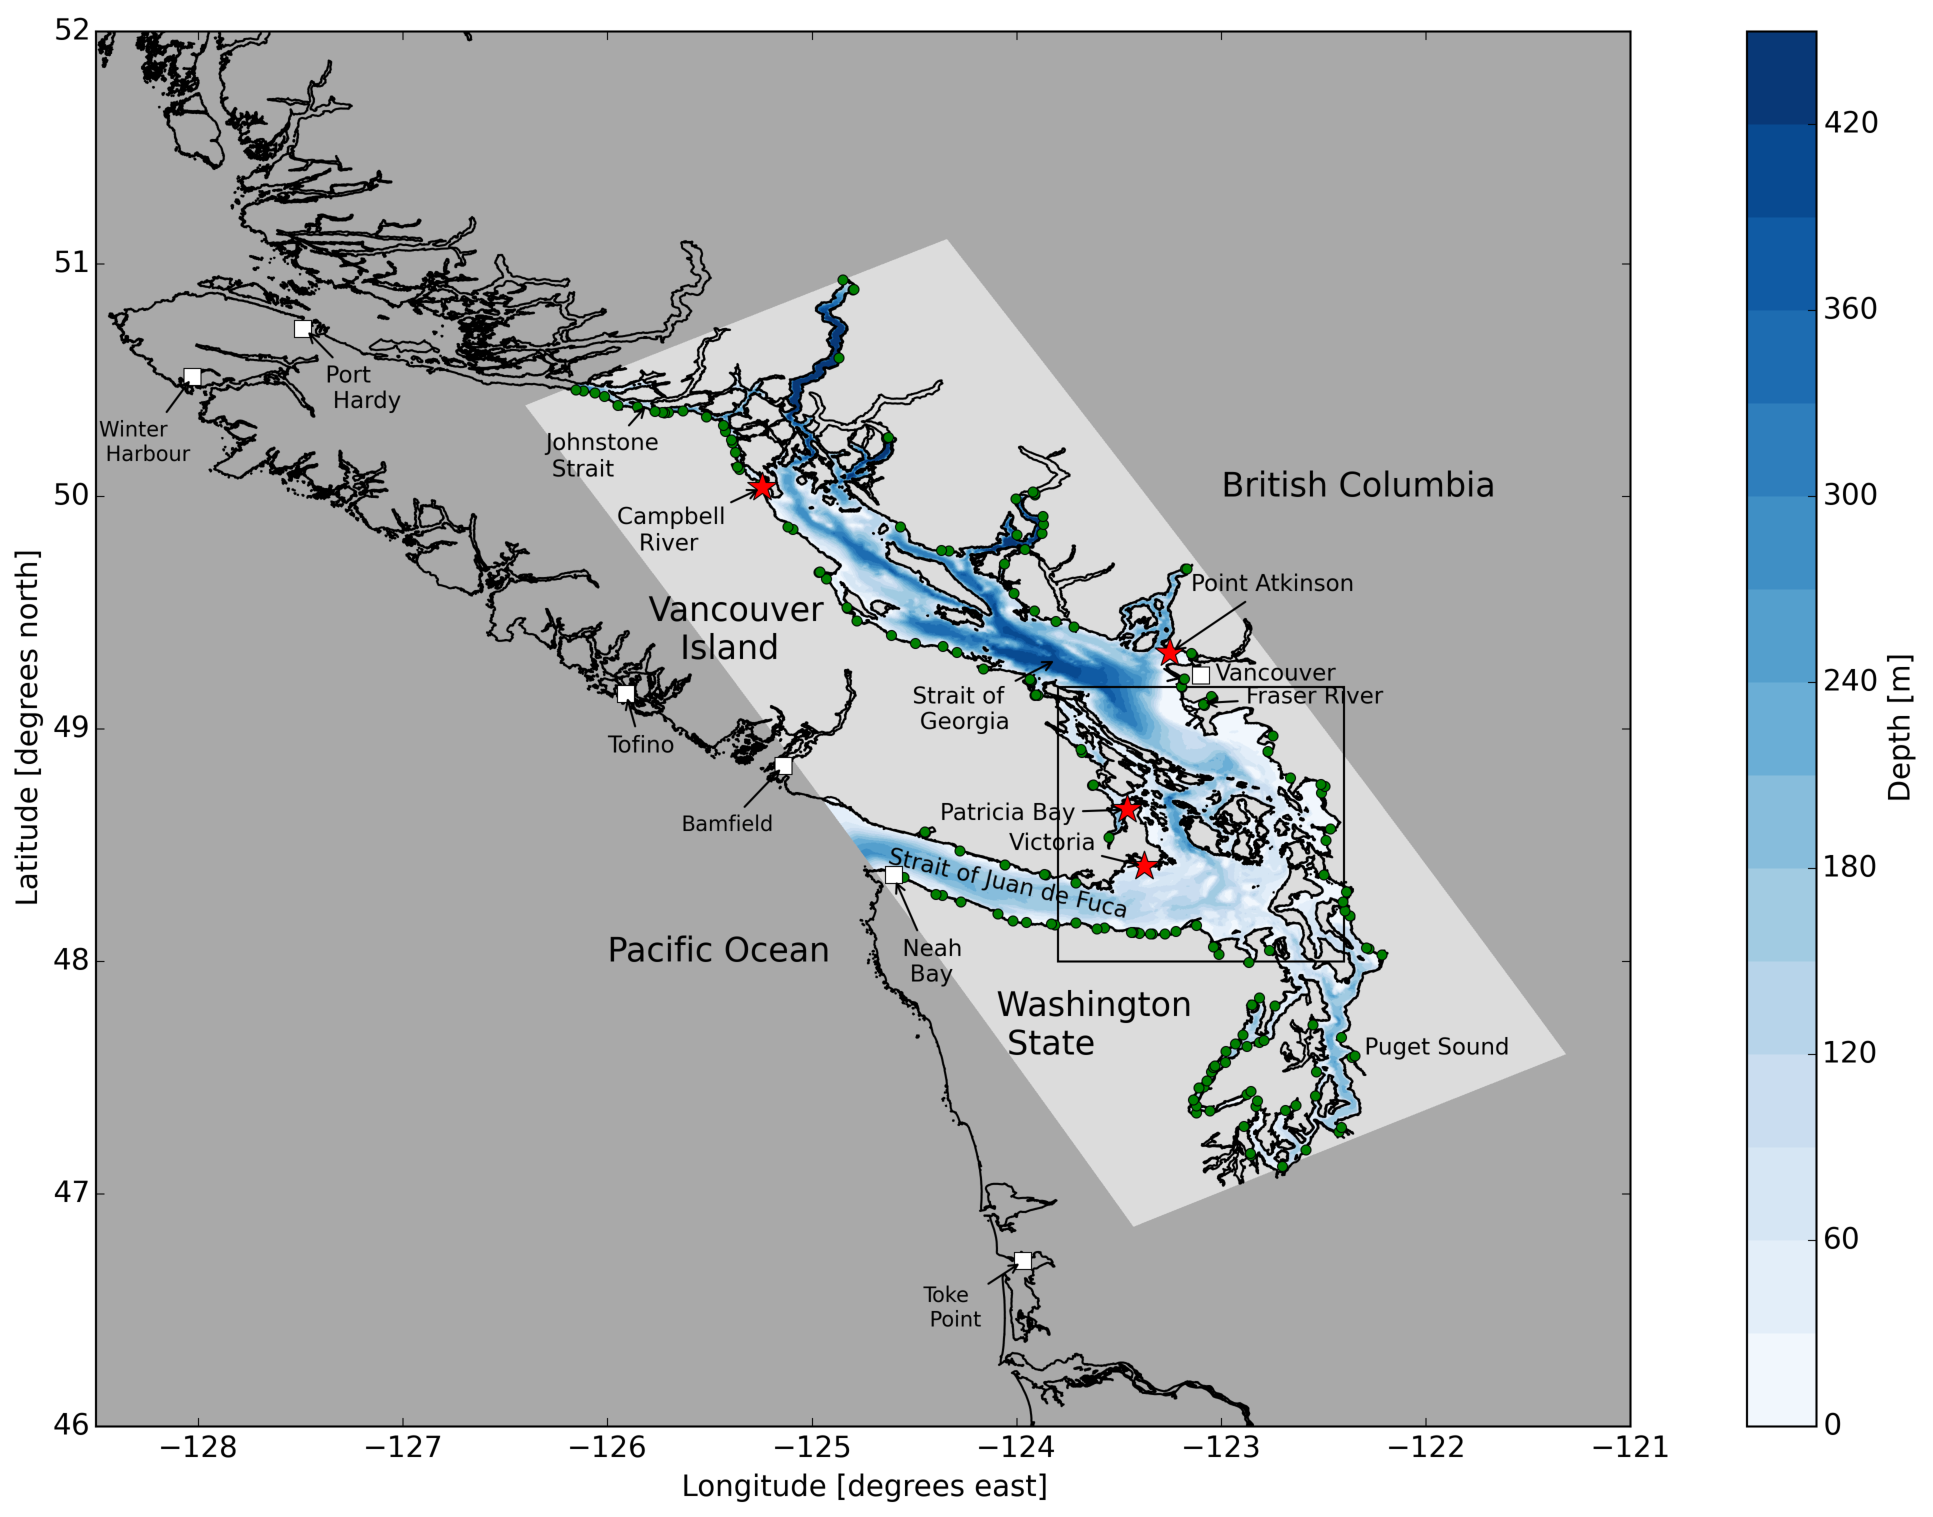
\includegraphics[scale=0.5]{Figures/bathy.pdf}
\caption{Model domain (highlighted area) including bathymetry, rivers (blue circles), and storm surge locations of interest  (red stars).}\label{fig:domain}
\end{figure}
%image may need more work

The model includes two open boundaries that connect to the Pacific Ocean, the western boundary of the Strait of Juan de Fuca as well as Johnstone Strait at the north, both of which are forced with eight tidal constituents (K$_1$ ,O$_1$, P$_1$, Q$_1$, M$_2$, K$_2$, N$_2$, S$_2$), temperature and salinity climatologies, and the sea surface height anomaly. Tidal heights and currents at grid points along the Juan de Fuca boundary were extracted from Webtide, an online web prediction model for the northeast Pacific Ocean, which is based on work by \citet{foreman2000webtide}. The Johnstone Strait boundary was forced with current and elevation tidal harmonics measured and calculated by \citet{thomson1980johnstone} for the major M$_2$ and K$_1$ constituents. Additionally, O$_1$ and S$_2$ elevation harmonics from their measurements were employed. The remaining constituents were extrapolated from Webtide. 
% Needs editing! Update when we are finished with tides.

Temperature and salinity at the Juan de Fuca boundary were taken from a weekly climatology which was created from results from a model covering the Salish Sea and the west coast of Vancouver Island \citep{massonfine2012}.  Their results, originally on s-levels were interpolated onto z-levels and then onto the NEMO horizontal grid.  To prepare the climatology all years (1995-2008) were averaged and results, approximately every 15 days, were interpolated to a weekly climatology. The model is relaxed to the forced temperature and salinity over the 10 grid points (about 5km) closest to the open boundaries, using a flow relaxation scheme \citep{engedahl1995use}. %other references?

Sea surface height at the mouth of Juan de Fuca was set using values from the Tofino tide gauge.  A monthly climatology was produced using daily averages from 2000-2010, binning them by month, averaging and setting the yearly mean to zero.  For the storm surge simulations, hourly variations in sea surface height were used.  These values are the Tofino tide gauge values, de-tided and with the zero reset as for the climatology. The storm surge simulations also used the sea surface height anomaly from Port Hardy, forced at the northern boundary in Johnstone Strait. The tidal forcing and sea surface height was used in the barotropic velocity forcing which used the NEMO Flather scheme \citep{flather1994storm, madec2012nemo}.
The baroclinic velocities at the boundary were set to be equal to the values inside the boundary (zero-gradient boundary conditions).  This scheme is not part of core NEMO.  Zero gradient conditions were chosen because the baroclinic velocity at the mouth of Juan de Fuca is primarily estuarine and thus set by density variations between inside and outside the domain.

At coastal boundaries, the partial slip boundary condition, an approximation to no slip, is used. Partial slip allows one to include the frictional effects of lateral boundaries without the restrictive resolution required to represent the lateral boundary layer under no slip conditions. A lateral eddy viscosity of 20 m $^2$ s $^{-1}$ parametrizes horizontal friction and a lateral eddy diffusivity of 20.5 m $^2$ s $^{-1}$ is used.  Bottom friction is represented by a quadratic law for the bottom momentum flux with drag coefficient $C_D = 5\times 10^{-3}$. Vertical turbulence and mixing is calculated through the $k-\epsilon$ configuration of the generic length scale (GLS) turbulence closure \citep{umlauf2003generic} with background vertical eddy viscosity and diffusivity set to $1\times10^{-4}$ and $1\times10^{-5}$ m$^2$ s$^{-1}$ respectively. Details on the NEMO implementation of the partial slip lateral boundary condition, quadratic bottom friction law, and GLS turbulence closure scheme are provided by \citet{madec2012nemo}.

At the ocean surface, meteorological conditions and fresh water input from rivers are included. The ocean surface is forced with momentum and heat fluxes from a 33-km global atmospheric reforecasting model suitable for use in ocean modelling \citep{smith2013new}. Forecasts from the period of 2002-2011 are available. Additionally, the inverse barometric effect of the atmospheric pressure is included, an important consideration in storm surge modelling. 

River input provides a significant volume of freshwater to the Salish Sea and can influence stratification, circulation and primary productivity. However, most rivers in the domain are not gauged so parametrizations were required to represent river flow. \citet{morrison2011rivers} provides a method for estimating freshwater runoff in the Salish Sea region based on precipitation. Monthly runoff volumes for each watershed for each year from 1970 to 2012 were acquired from \citet{morrison2011rivers}, as well as monthly averages. 

Freshwater runoff from each watershed was divided between the rivers in that watershed. The area drained by each river was estimated from Toporama maps by the Atlas of Canada and watershed maps available on the Washington State government website. The watersheds included in our model were Fraser (which represents approximately 44\% of the freshwater input into our domain), Skagit (12\%), East Vancouver Island (North and South) (12\%), Howe (7\%), Bute (7\%), Puget (6\%), Juan de Fuca (5\%), Jervis (4\%) and Toba (3\%). 

The monthly flow from each river was input as a point source in the three grid points closest to the surface at the model point closest to the mouth of each river. Incoming water was assumed to be fresh and at surface temperature. A total of 150 rivers were parametrized by this method and their locations are indicated by the blue dots in Figure \ref{fig:domain}.

Initial conditions for temperature and salinity were taken from a CTD cast in the middle Strait of Georgia taken in Sept 2002 \citep{pawlowiczetal2007}.  Conditions were initially uniform horizontally and velocity was initialized at zero. The model was spun up for a 15.5 months from the initial conditions above, starting Sept 16, 2002, using atmospheric forcing from 2002-2003, climatological temperature and salinity and sea surface height at the boundaries, with tides and climatological river output.  All storm surge runs were started three days prior to the event of interest with zero initial velocities and sea surface height and a stratification profile from model spin up. The modelled sea surface height adjusted to forcing in less than one day. 

\section{Model Evaluation}\label{sec:model}

\subsection{Tidal evaluation}
The model was initially evaluated qualitatively by comparing patterns of tidal amplitude and phase to results from \citep{foreman1995tidal}. For example, the amphidrome around Victoria was produced in the M$_2$ results, as well as the monotonic increase in $K_1$ amplitude moving northwards along the Strait of Georgia. Initially, the Johnstone Strait boundary was closed, but modelled M$_2$ amplitudes were too small compared to measured amplitudes... TBC

%perhaps a nice contour map of M2 and K1 amps and phases goes here?

Once our model was reproducing observed tidal patterns, model results were quantitatively evaluated by comparing modelled harmonic constituents to measured harmonic constituents at tidal measuring stations throughout the domain. Comparisons were made using the complex difference ($D$), defined by \citep{foreman1995tidal} as:

\begin{equation}
D = [(A_0 \cos g_0 - A_m \cos g_m)^2 + (A_0 \sin g_0 - A_m \sin g_m)^2]^{1/2}
\end{equation}\label{eq:compdiff}
where $A_0$, $A_m$, $g_0$ and $g_m$ are observed and modelled amplitudes and phases.

%perhaps a table of complex differences at tidal stations similar to Table 1 of Foreman et al (1995)  (such as the one produced by tidetools.calc_diffs_meas_mod) here?
%(would be cool to include the complex differences calculated at the VENUS nodes too)



Complex differences were less than ??cm at all stations in our domain, which was assumed to be acceptable for our purposes. 
%if it's favourable, we could compare our complex differences to Foreman et al (1995), who got an average of D=3cm for M2 and D=2.5cm for K1

\begin{figure}
\centering
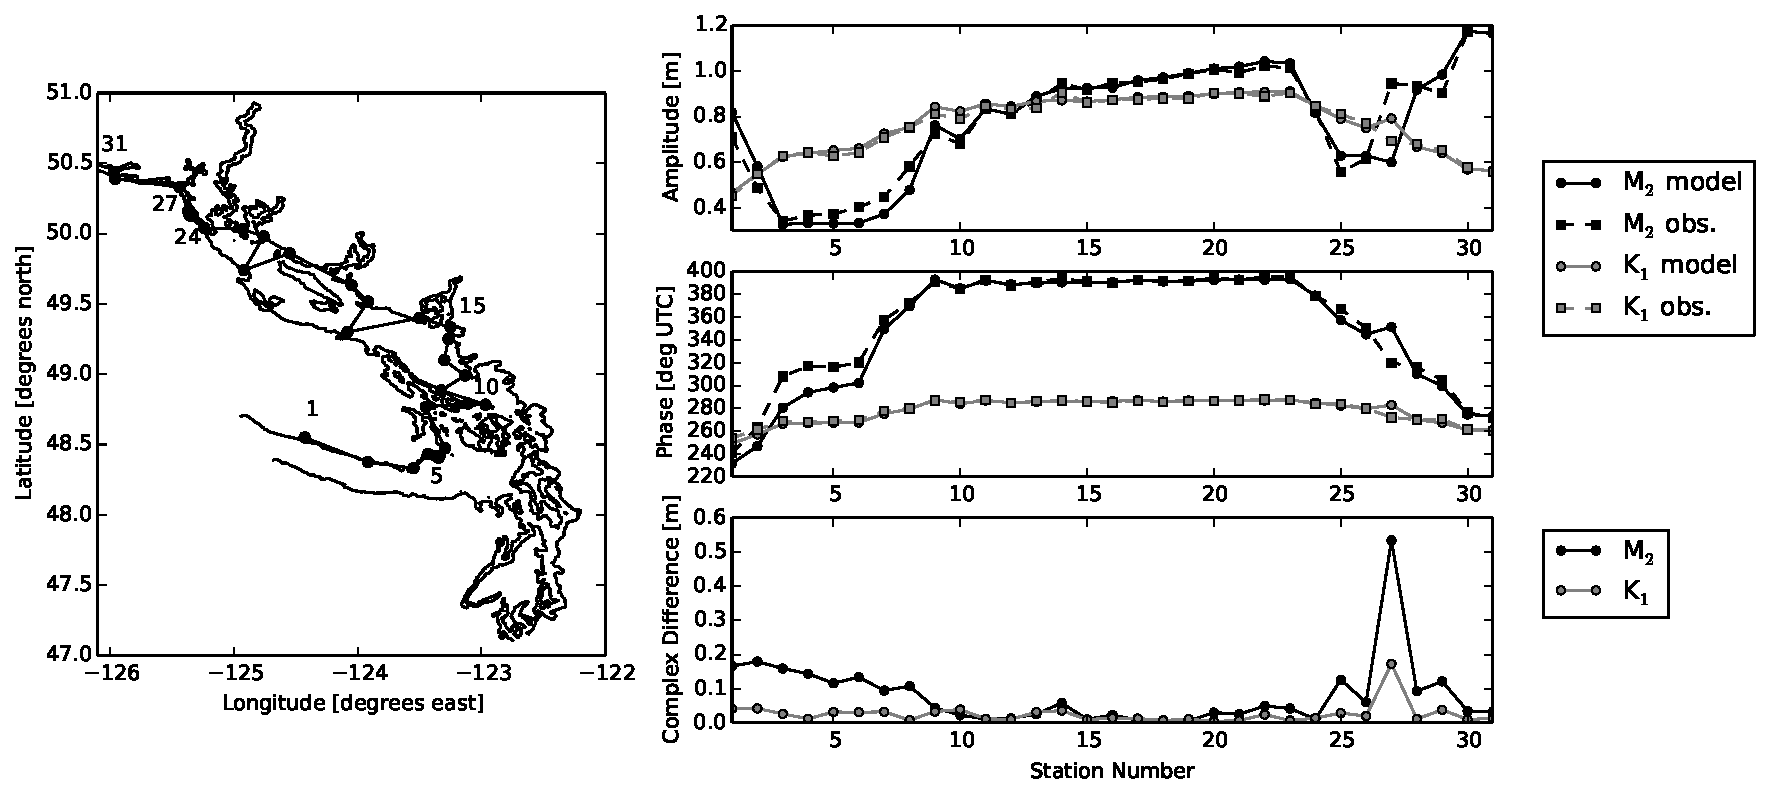
\includegraphics[scale=0.6]{Figures/tides.pdf}
\caption{Evaluation of model tidal amplitude and phases for the M$_2$ and K$_1$ constituents. On the left, a transect through the stations used for comparison. On the right, modelled M$_2$ (black) and K$_1$ (gray) amplitude (top) and phase (middle) compared with observations in the dashed curves of the same colour. The bottom plot displays the M$_2$ and K$_1$ complex differences.  }
\label{fig:tides}
\end{figure}


\section{Storm Surge Hindcasts}\label{sec:storm}
%outline: 
%1. factors contributing to storm surge with focus on Feb 2006 event
%2. Strong wind event but no surge (maybe Dec 2006 or Nov 2009)
%3. High resolution wind (hopefully Dec 2012)
A series of storm surge hindcasts is presented next. Storm surge simulations were started from rest at least three days prior to the event of interest to allow for adjustment of model currents. Stratification conditions from model spin-up at a time close to the event (within 5 days) were chosen to initialize the temperature and salinity fields. Boundary conditions include atmospheric forcing and fresh water input from rivers at the surface, sea surface height anomaly from observations at the open boundary, and tidal forcing with eight tidal constituents. Forcing the model with only eight tidal constituents leads to an error in modelled sea surface height predictions due to the omission of the next leading order tidal constituents such as J$_1$. Comparisons between full tidal predictions and tidal predictions using eight constituents suggest that this error can be up to 40 cm (check) during times of high tidal range, and in particular, during the storm surge season Nov-Feb. As such, storm surge model predictions were corrected by accounting for this error. Additionally, since the sea surface height is calculated about a zero reference level, the modelled water level is determined by adding a long term average of mean sea level at the specified location to the modelled sea surface height.

Model results have been compared with observations by calculating both the total modelled water level and the modelled residual. The modelled residual is calculated as the difference in model output between a simulation with all forcing conditions and a simulation forced only with tides and rivers. Water level observations are taken from Fisheries and Oceans Canada (citation) and are used to calculate the osberved residual, defined as the observed water level minus tidal predictions. Tidal predictions are calculated using t\_tide \citep{pawlowicz2002classical}, a MATLAB tool that calculates tidal harmonics from a given time series, in this case, from the year prior surge event of interest. Additionally, several simulations with varying forcing conditions such as removing atmospheric forcing or removing the sea surface height anomaly at the open boundaries have been completed. 

Several significant surge or wind events have been considered in detail, as well as an array of hindcasts to asses model ability in a statistical measure. These cases have been used to asses the model's skill in reproducing water level height and surge amplitude and timing during storm events. In addition, the contribution to the surge due to several forcing conditions, such as atmospheric forcing and open boundary forcing, has been assessed. We have also examined the spatial variability of the surge as it propagates through the domain and have considered a case with high-resolution atmospheric forcing. 

The model's skill is reported through a few statistical measures of the the total water level $\eta$ and the residual $\delta$. First, the mean absolute error ($\bar{e}$), defined as
\begin{equation}
\bar{e} = \text{mean}\left(\left| M - O \right|\right),
\end{equation}
where $M$ and $O$ are the modelled and observed quantities of interest, is a common measure that estimates the average error in the model. Next, a measure comparing the variance of the error to the variance of the observations defined as \citep{thompson2003prediction},
\begin{equation}
\gamma^2 = \frac{\text{var}\left(M-O\right)}{\text{var}\left(O\right)},
\end{equation}
is also calculated. Smaller values of $\gamma^2$ indicate better model skill. This quantity was used by \citet{bernier2006predicting} and \citet{bernier2010tide} in storm surge predictions in Eastern Canada and is caclulated here as a point of comparison. A third measure, called the Willmott skill score \citep{willmott1982some}, is also used to assess overall model skill in predicting the water level and residual. This quantity is defined as
\begin{equation}
WS = 1 - \frac{\sum_{i=1}^N \left(M_i - O_i\right)^2}{\sum_{i=1}^N \left(|M_i'| + |O_i'|\right)^2},
\end{equation} 
where $M_i' = M_i-\bar{O}$ and $O_i'=O_i-\bar{O}$ and $\bar{O}$ is the mean of the observations. This score is bounded by zero and one. Values close to one indicate good model skill. 

%First, a study of a large surge event on Feb 4, 2006 is presented. This event caused significant damage and flooding in Boundary Bay, a community south of Richmond, (citation) and has been chosen as a case study to demonstrate the model's skill in reproducing a storm surge and to quantitatively assess forcing conditions that are important in storm surge hind casting. Second, an extreme wind event on Dec 15, 2006 is examined. This event produced winds over (x) (citation) but did not result in significant flooding because the storm did not occur at high tide, however, it did result in significant property damage due to high winds and waves. This event has been used to understand the spatial and temporal variability of the surge propagation. Next, a large wind event on Nov 18, 2009 that did not result in a significant surge or flooding is presented. This case was chosen to identify the model's capability in handling large wind events that do not result in high water levels. Next, a case with high resolution atmospheric forcing for a recent surge on Dec 17, 2012 is discussed. Lastly, these cases presented in detail will be combined with $x$ additional runs for statistical evaluation of model performance. 


\subsection{Factors Contributing to Storm Surges: Feb 4, 2006}

On Feb 4, 2006, a strong storm system with winds over 75 km/hr coinciding with an unusually high tide led to significant flooding in coastal communities of the Strait of Georgia \citep{romanowski2010storm}. The maximum water level observed at Point Atkinson on this day was 5.46 m, which is 0.82 m higher than the predicted tides, highlighting the significance of this event as it resulted in a large anomaly and also reached water levels close to the highest level ever recorded (5.61 m). A set of simulations from Feb 1 to 8, 2006 under a variety of forcing conditions has been completed in order to determine the contribution of each forcing factor to the surge.

The model's ability to reproduce this event is demonstrated in Figure \ref{fig:feb2006} which compares observations and corrected model output at Point Atkinson, Victoria, Patricia Bay, and Campbell River. The timing of maximum water level matches well between the observations and the model at all four locations, the most significant contribution to high water level being from the tides which are generally well-represented by the model. There is a good match in the water level maximum at Victoria and Patricia Bay, with a relative error less than 2\%. There is only a 4.2 cm difference between observed and modelled water level elevation at Victoria and a 6.9 cm difference at Patricia Bay, the model slightly underpredicting the maximum water level in each case. The error at Point Atkinson and Campbell River is slightly more significant, reaching 2.5\% and 2.7\% respectively, close to 14 cm overpredicted in each case. It is suprising that Victoria and Patricia Bay agree most closely with observations because the M$_2$ tidal amplitudes in the model are known to be too low in this area. In conjunction with the overpredicted water levels at Point Atkinson and Campbell River, it is likely that one of the forcing factors is overestimated in this example. 

A comparison between observed and modelled residuals is also displayed in the panels on the right. In general, there is a very good agreement between the observed and modelled residules. The most noticeable difference is a 4-6 hour delay in the model's timing of the maximum residual except at Victoria where the maximum residual in sync with observations. The errors in maximum residual range from 6.0 cm to high at Victoria to 15.9 cm too low at Campbell River. Point Atkinson and Patricia Bay both experience a very good match with observed residuals with errors less than 2 cm. Note that Point Atkinson and Campbell River observed the largest observed surges at 82 cm and 95 cm respectively. The surges at Victoria and Patricia Bay were observed to be 66 cm and 74 cm. 


\begin{figure}
\centering
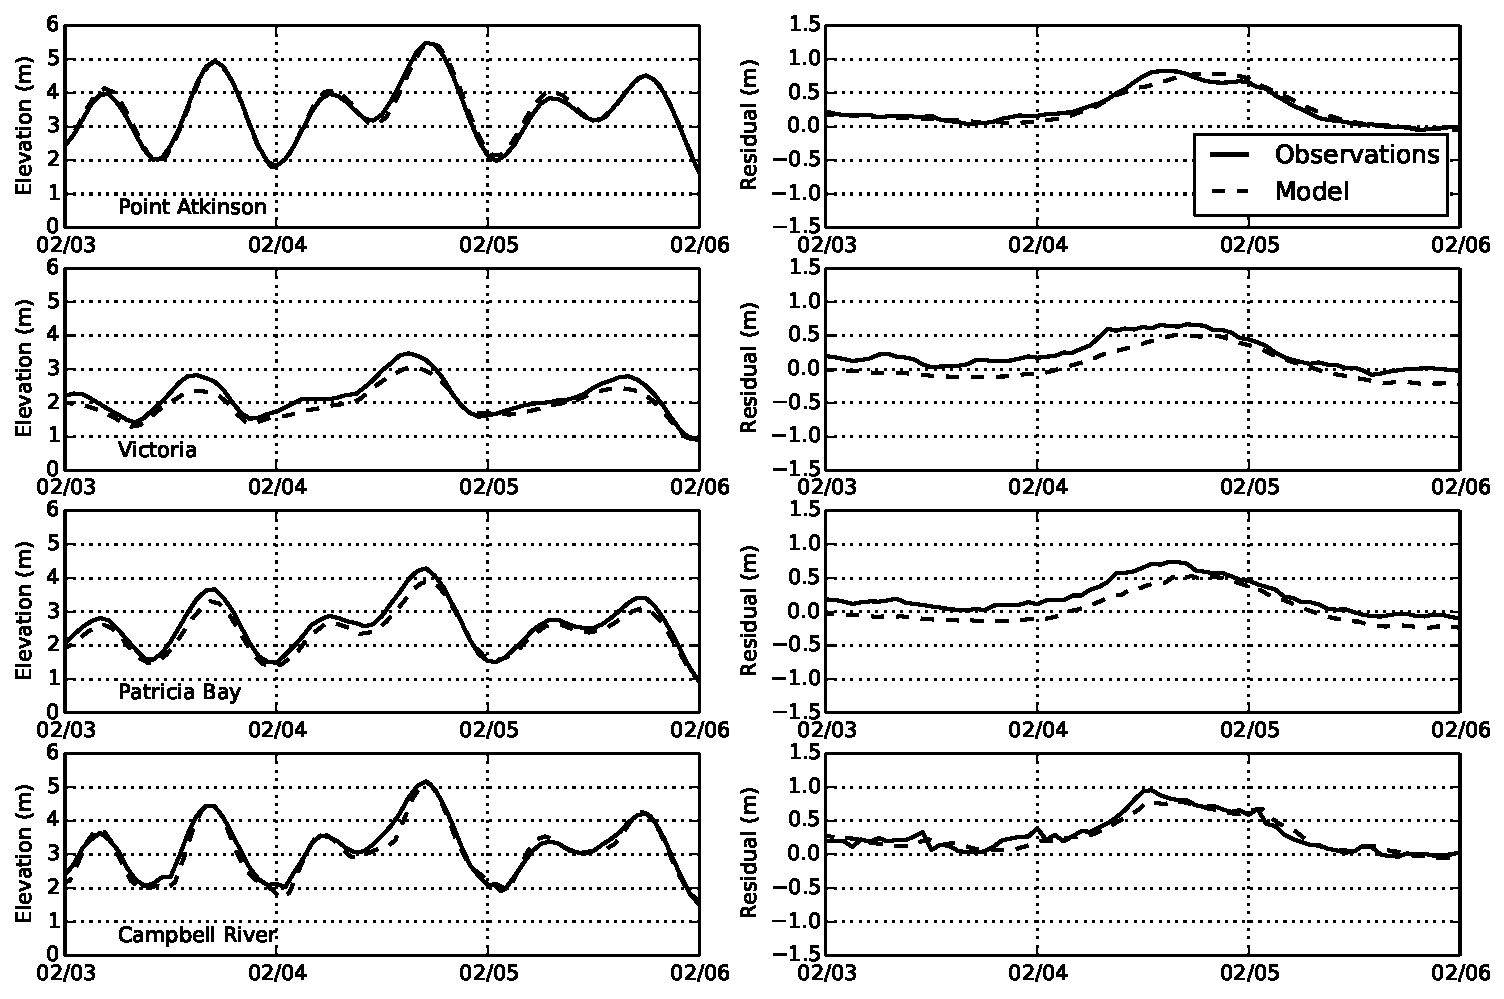
\includegraphics[scale=0.6]{Figures/feb2006.pdf}
\caption{Comparison of observations and model output for the Feb 4, 2006 storm surge. Left: total water level observation (solid) and corrected model (dashed). Right: observed residuals (solid) and modelled residuals (dashed).}
\label{fig:feb2006}
\end{figure}

The maximum water level and maximum residuals are important factors in storm surge hindcasts but a better indicator of overall model performance is provided by a group of statistical measures in Table \ref{tab:feb2006stat}. In general, $\gamma^2$ and $WS$ suggest good model agreement for the predicted water levels, most likely because the tidal signal dominates. The skill scores degrade slightly for the residuals but are still reasonable and indicate very good agreement. Note that the mean absolute error ($\bar{e}$) is lower for the residuals, but this measure does not account for the larger variablity in water levels due to the tides.

\begin{table}[h]
\centering 
\begin{tabular}{|l |c c c | c c c|} 
\hline 
& \multicolumn{3}{|c|}{Water Level ($\eta$)}        & \multicolumn{3}{|c|}{Residual ($\delta$)} \\ 
\hline 
Location       & $\bar{e}$ (cm) & $\gamma^2$ & $WS$   & $\bar{e}$ (cm) & $\gamma^2$ & $WS$      \\
\hline 
Point Atkinson & 10.5           &   0.012    & 0.994  & 6.2            &  0.065     & 0.979     \\
Victoria       &  8.6           &   0.032    & 0.992  & 6.1            &  0.085     & 0.970     \\
Patricia Bay   &  9.1           &   0.024    & 0.992  & 6.9            &  0.070     & 0.969     \\
Campbell River & 13.1           &   0.041    & 0.990  & 5.8            &  0.079     & 0.961     \\
\hline 
\end{tabular}
\caption{Evaluation of model performance for the Feb 2006 simulation. Mean absoulte error ($\bar{e}$), $\gamma^2$, and the Willmott skill score ($WS$) are provided for water level predictions ($\eta$) and resdiuals ($\delta$) during the period displayed in Figure \ref{fig:feb2006}.}
\label{tab:feb2006stat} 
\end{table} 
%anything else to include? statistics calculated in Feb 2006 -paper prodcution.ipynb and saved in statisitcs_feb2006.csv 
%mean of model and mean of observations?

Next, an assessment of the factors that are most important in scenarios leading up to storm surges is presented in Figure \ref{fig:factors}. The modelled residual from four simulations have been plotted. First, a simulation with all the forcing conditions, including tides, atmospheric forcing, rivers, and sea surface height anomaly, is shown in the dashed black curve. Additionally, a simulation with all forcing except the atmospheric forcing is presented in solid grey and a simulation with all forcing except the sea surface height anomaly is shown solid black. Finally, a simulation with only wind forcing, that is no anomaly and no inverse barometer effect due to pressure, is shown in the dashed grey curve. It is clear that the sea surface height anomaly contributes most significantly to the surge at each of these locations. When the sea surface height anomaly is not included as a forcing condition, the surge drops from a maximum 82 cm to 11 cm at Point Atkinson and its maximum occurs eight hours later.  A similar drop in the maximum surge and delay in timing of the maximum surge is observed at the other locations. The atmospheric model indicates southeasterly winds near Point Atkinson during the onset of the surge but after the peak surge has passed, the winds shift to westerly. A strong westerly wind would cause an elevated sea surface height at Point Atkinson as water piles against the coast, explaining the delay in peak surge when only atmospheric forcing is used since the winds shift to westerly after the peak surge has passed. A simulation with only wind forcing produces a surge of 7.8 cm at Point Atkinson, a small fraction of the total observed surge, and only centimeters at the other locations. Note that this wind-induced surge occurs well after the peak surge from observations and simulations with full forcing.

The contribution to the surge due to atmospheric forcing appears to be geographically dependent, its removal leading to a drop of about 2.5 cm in the maximum surge at Point Atkinson and 2.3 cm at Campbell River. Interestingly, the surge amplitude increases by 4.8 cm at Victoria and 3.6 cm at Patricia Bay when atmospheric forces are negelcted. The southeasterly winds over the Strait of Georgia could be acting to push water away from the southern tip of Vancouver Island, resulting in slight decrease in the surge amplitude at Victoria and Patricia Bay when wind effects are included in the model. Additionally, the surge amplitude decreases by a few centimtres if the inverse barometer effect due to atmospheric pressure is not included. 

These comparisons point to the importance of including, as a forcing condition at the open boundary, the surge entering the domain from the Pacific Ocean. Storms travelling over the Pacific Ocean towards the west coast of the northern United States and Canada can induce elevated sea levels along the coastline which then enter the Salish Sea system through the Strait of Juan de Fuca. In a model domain that does not include the Pacific Ocean, this effect must be included as a boundary condition. Previous simulations by \citet{murty1995storm} suggest that the inverse barometer effect and the surge entering the system through the Strait of Juan de Fuca contribute most significantly to storm surges in this domain.  A detailed assessment of the effect of the local atmospheric conditions and winds should be performed with high resolution atmospheric forcing data.  

\begin{figure}
\centering
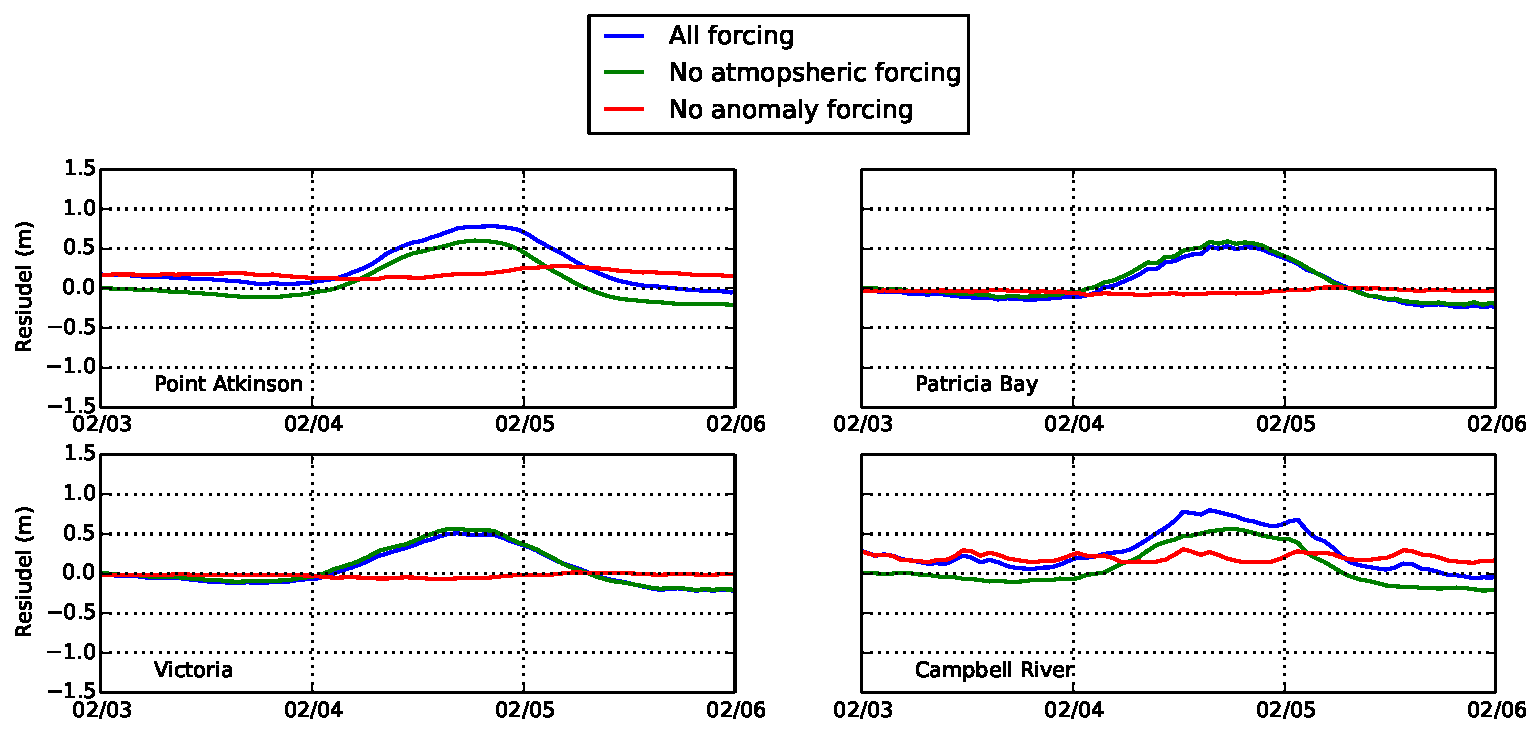
\includegraphics[scale=0.6]{Figures/feb2006_factors.pdf}
\caption{Comparison of the modelled residual for four simulations: A simulation with all forcing (solid black), a simulation without atmospheric forcing (solid grey), a simulation without the sea surface height anomaly (dashed black) and a simulation with only wind forcing, i.e.\ no sea surface height anomaly or pressure (dashed grey). }
\label{fig:factors}
\end{figure}

Finally, an assessment of the importance of including the tide-surge interaction is presented next. A simulation of the surge propagation without including any tidal forcing is compared with the modelled residual in Figure \ref{fig:tidesurge}.  Recall, the modelled residual is defined as the difference between the sea surface height in a simulation with all forcing and a simulation with tides and rivers only. A comparison between the modelled residual and a surge-only run can determine the significance of the tide-surge interaction. The most significant differences occur at Point Atkinson where the maximum of the surge-only case is 8.7 cm higher than maximum modelled residual, about 10\% higher of the surge amplitude.  In contrast, the tide-surge interaction at Victoria is hardly noticeable. Indeed, a spatial map of the difference between the modelled residual and surge-only difference (not shown here) indicates that the tide-surge interaction is more pronounced after the San Juan and Gulf Islands. The passages between these islands are known for vigorous tidal mixing, which may have a nonlinear effect on the surge propagation. However, the effect is a relatively small overestimate of the surge elevation and no changes to the timing of the surge. So, in operational settings, performing a surge-only simulation and adding the predicted tides a posteriori could be more computationally efficient with only a small decrease in the accuracy of the prediction. 

\begin{figure}
\centering
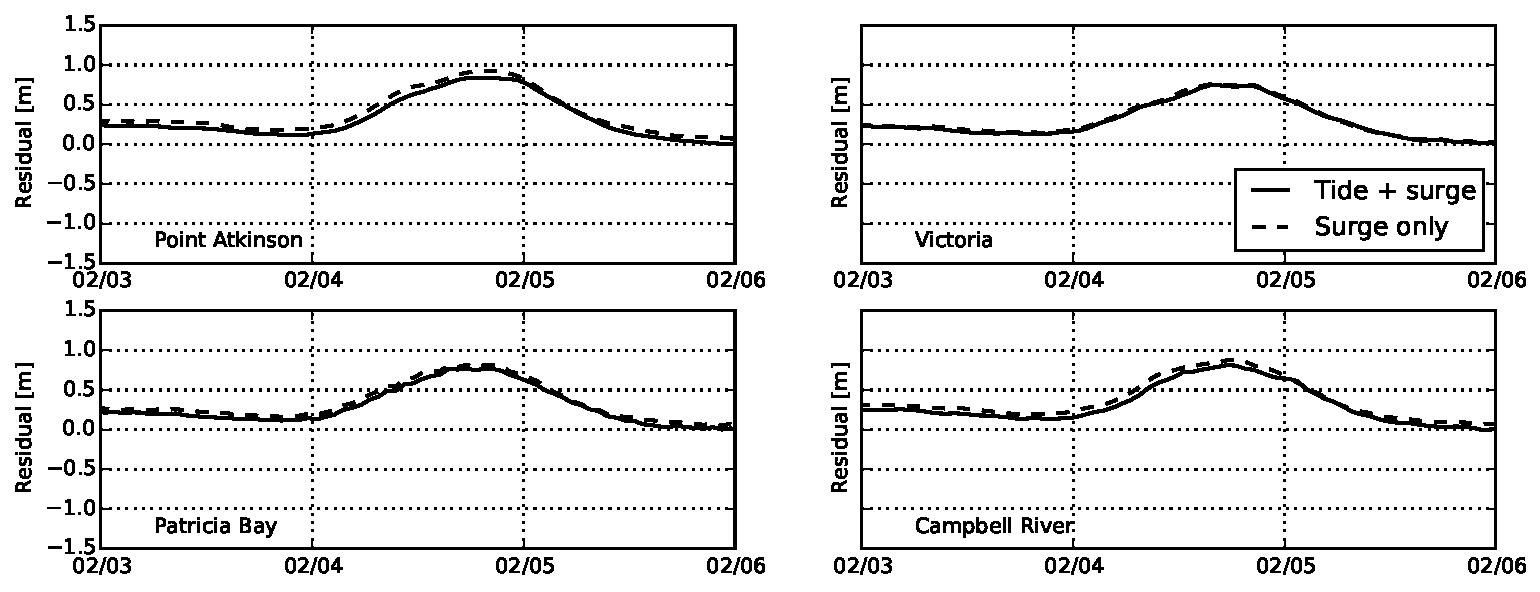
\includegraphics[scale=0.6]{Figures/feb2006_tidesurge.pdf}
\caption{Modelled residuals (solid) compared with a simulation of the surge propagation without tidal forcing (dashed). }
\label{fig:tidesurge}
\end{figure}

\subsection{Spatial Extent of Surge: Dec 15, 2006}
On Dec 15, 2006, a major storm with wind gusts over 120 km/hr caused significant damage to many coastal communities on the Pacific Northwest. Although the storm was very strong and the observed residual at Point Atkinson reached 84 cm, this event did not coincide with high tide and so no significant or reported flooding occurred in the Vancouver area \citep{forseth2006adaptation}. This event has been used to examine the propagation of the surge throughout the domain and spatial variations in the surge amplitude. First, an assessment of the accuracy of the hindcast is provided. 

Point Atkinson observed a maximum surge amplitude of 84 cm, which is approximately 28 cm higher than the modelled residual, however the timing of the surge agrees almost exactly as displayed in Figure \ref{fig:dec2006}. The best agreement occurs at Victoria where the observed surge was 62 cm and the model returned 44 cm. At all of the locations, the model predicted the maximum surge to occur within 3.5 hours of the observed surge. Typically, the modelled surge was too early, in contrast to the later predictions in the Feb 4, 2006 case. Error and skill scores for the modelled water level and the modelled residual are provided in Table \ref{dec2006stat}. The modelled residuals are on average too low and have a lower skill score than the Feb 2006 case. This could be due to a number of factors. First,the very large wind speeds observed during this storm are significantly underrepresented by the atmospheric model leading to lower wind stress and less piling of water against the coast. Second, the anomaly forcing at the open boundaries could be too low. The observed residual at Tofino, BC (a point near by but outside of the domain) is up to 10 cm lower than the observed residual at Neah Bay, WA (a point near by but inside of the domain). Since the storm surge is less sensitive to wind forcing at the surface than anomaly forcing at the open boundaries, the latter is likely the case. 
%Skill score between CGRF and observed winds? 

\begin{figure}
\centering
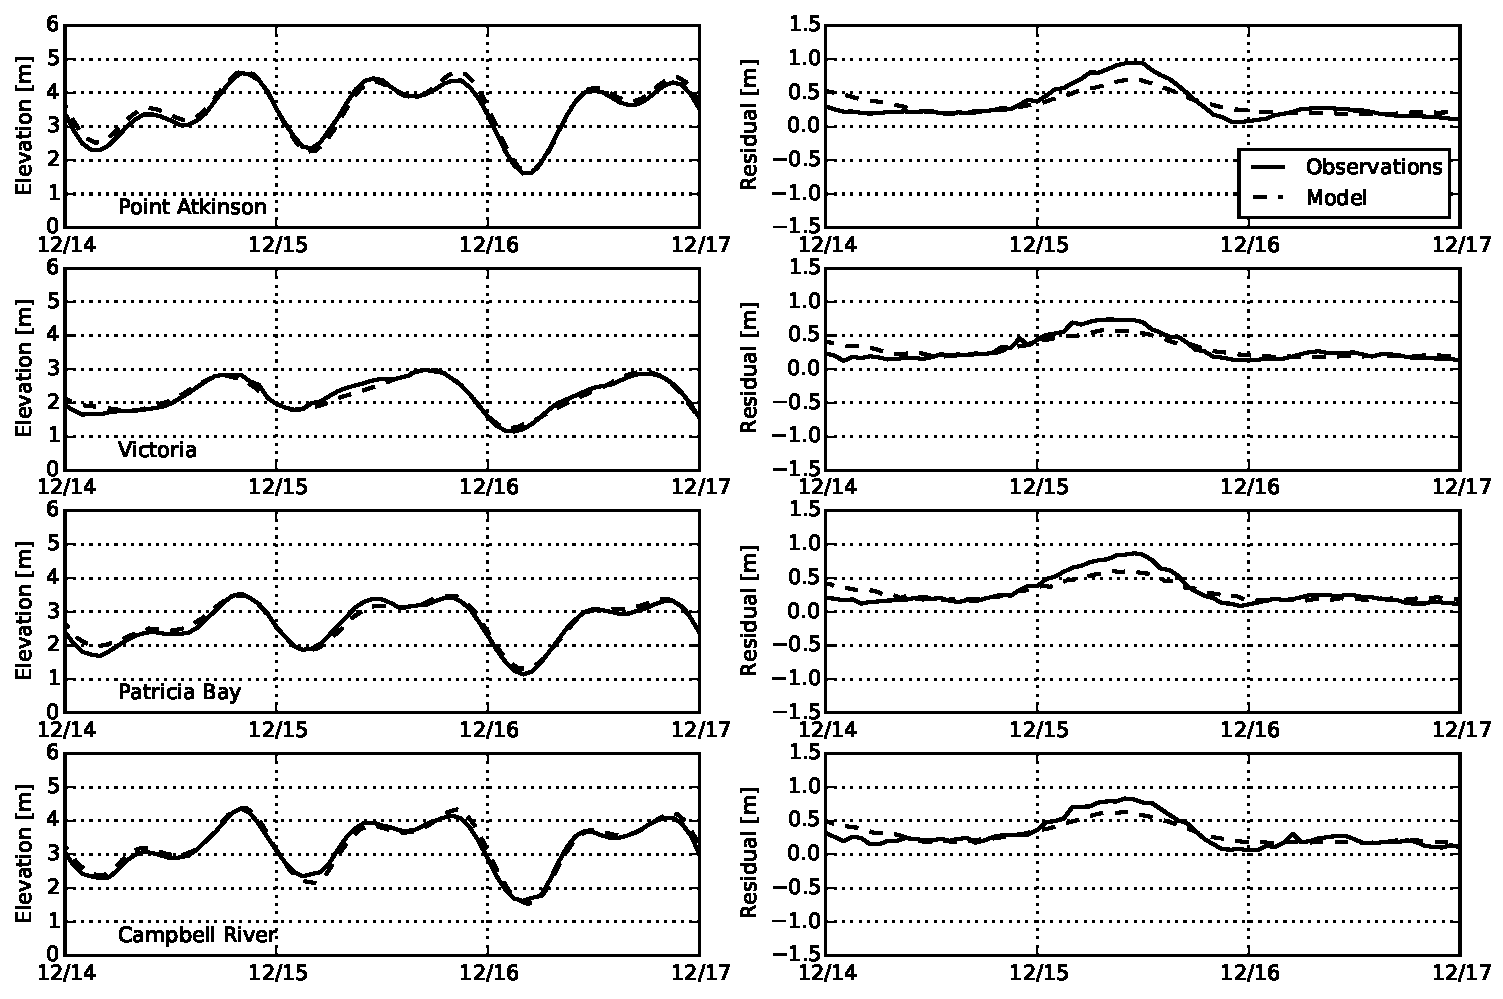
\includegraphics[scale=0.6]{Figures/dec2006.pdf}
\caption{Comparison of observed and modelled water level and residuls during the Dec 15, 2006 storm surge simulation. }
\label{fig:dec2006}
\end{figure}%table instead of figure?

\begin{table}[h]
\centering 
\begin{tabular}{|l |c c c | c c c|} 
\hline 
& \multicolumn{3}{|c|}{Water Level ($\eta$)}        & \multicolumn{3}{|c|}{Residual ($\delta$)} \\ 
\hline 
Location       & $\bar{e}$ (cm) & $\gamma^2$ & $WS$   & $\bar{e}$ (cm) & $\gamma^2$ & $WS$      \\
\hline 
Point Atkinson & 10.5           &   0.025    & 0.994  & 11.1           &  0.275     & 0.891     \\
Victoria       &  9.6           &   0.042    & 0.984  &  7.9           &  0.223     & 0.911     \\
Patricia Bay   &  9.2           &   0.031    & 0.990  &  9.5           &  0.260     & 0.889     \\
Campbell River & 10.6           &   0.030    & 0.992  & 10.6           &  0.247     & 0.905     \\
\hline 
\end{tabular}
\caption{Evaluation of model performance for the Dec 2006 simulation.}
\label{tab:dec2006stat} 
\end{table}

The evolution and spatial distribution of the surge is highlighted in Figure \ref{fig:spatial} where the modelled residual is plotted every hour beginning on Dec 15 at 05:30 UTC through to Dec 15 at 14:30 UTC. The surge enters the system from the Strait of Juna de Fuca, peaking between Dec 15 at 9:30 and Dec 15 at 11:30 and then begins to subside throughout the entire domain. Notably, the Strait of Georgia experiences the largest surge values, upwards of 60 cm, whereas the Juan de Fuca region experiences a maximum surge around 45 cm. Additionally, the coastal areas on the mainland side of the Strait of Georgia experience slightly higher surges than the Vancouver Island side, likely due to the southerly wind in the atmospheric model pushing water against the mainland coast. At about 11:30 UTC, the winds switch to northwesterly and then westerly, further amplifying the surge along the mainland coast. 

\begin{figure}
\centering
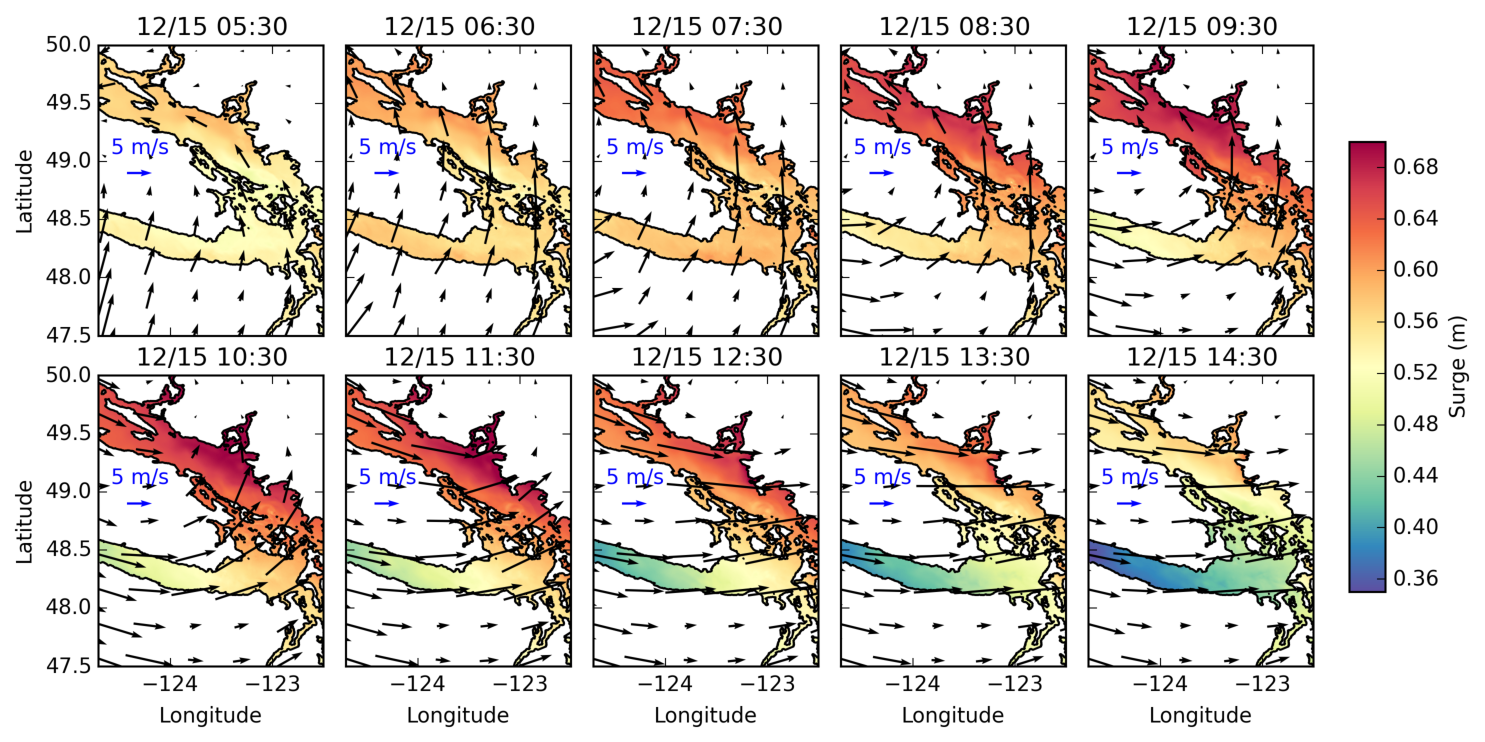
\includegraphics[scale=0.6]{Figures/dec2006_spatial.pdf}
\caption{Propagation of the storm surge on Dec 15, 2006. Modelled residual every hour starting on Dec 15 at 05:30 UTC. Time advances from top left to bottom right. Wind vectors from the atmopsheric forcing are overlaid in black.}
\label{fig:spatial}
\end{figure}

An evaluation of the spatial distribution of the surge in a simulation without atmospheric forcing is provided in Figure \ref{fig:spatial_sshonly}. In this case, the surge amplitude across the Strait of Georgia, is uniform with no pronouced difference between the mainland side and Vancouver Island side. While the surge entering the domain from the Pacific Ocean is the leading order contribution, the winds may induce localized changes to the surge amplitude. Interestingly, the winds over the Strait of Juan de Fuca cause a decrease in surge amplitude in this region as the winds are acting to push the water towards the mainland.  Even without atmospheric forcing, there is still a siginificant difference in surge amplitude between the Strait of Georgria and the Strait of Juan de Fuca, perhaps because the Strait of Georgia is also affected by the surge entering the domain from Johnstone Strait at the northern boundary.

\begin{figure}
\centering
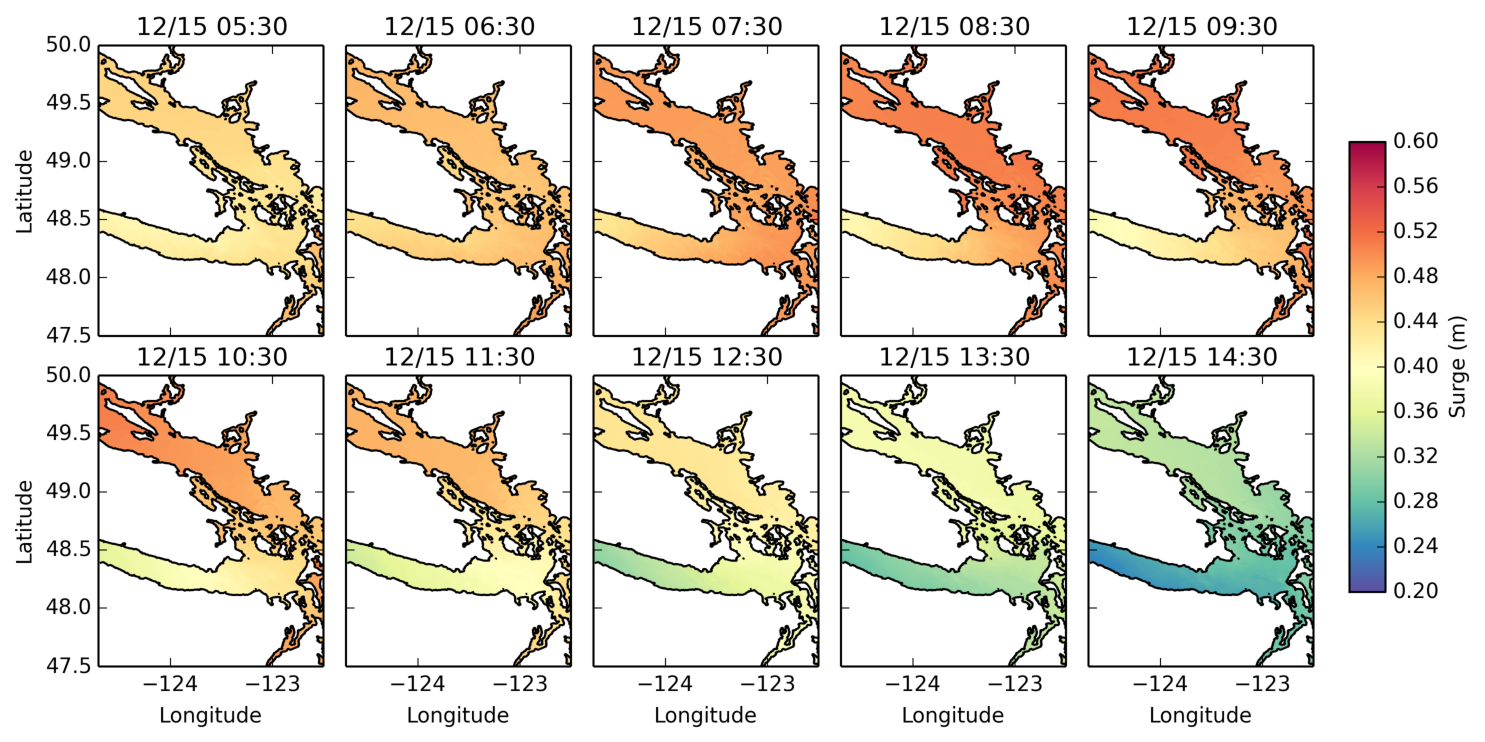
\includegraphics[scale=0.6]{Figures/dec2006_spatial_sshonly.pdf}
\caption{As in Figure \ref{fig:spatial} but for a simulation that does not include atmopsheric forcing. }
\label{fig:spatial_sshonly}
\end{figure}

\subsection{Strong Wind Event: Nov 19, 2009}
Next, a relatively strong wind event recorded at Point Atkinson on Nov 19, 2009 is considered. As recorded in the Environment Canada Historical Climate Data archives, the maximum hourly wind speed at Point Atkinson was 18.6 m/s and the largest gust observed was 25.8 m/s or 93 km/hr. In addition, large wind speeds over 15 m/s persisted for over 9 hours. Yet, the surge associated with this event is rather small when compared the previous two cases as shown in Figure \ref{fig:nov2009} where we have plotted the wind speed at Point Atkinson, sea surface height anomaly forcing at the open boundaries, and observed and modelled residuals at Point Atkinson. Two significant surge events are noted, the first occurring on Nov 19 and a second, larger surge on Nov 20. The largest surge did not coincide with the strong wind event which peaked at Nov 19 01:00 hr, reflected in both the model and observations. The highest observed surge reached 62.6 cm on Nov 20 at 10:00 hr, while the model recorded a maximum surge of 38.8 cm five hours later. The surge did not occur during a high tide and so no high water level events were recorded. Although not shown here, the other three locations also observed a maximum surge on Nov 20, which appears to be linked to a secondary high wind event and a more significant surge entering the system at Tofino and Port Hardy. 

\citet{danard2003storm} discuss the role of wind fetch, the distance over which wind acts on the surface of a water basin, in setting up seiche motion in lakes and its contribution to storm surges. As wind blows over the surface of a lake, the water level becomes elevated on the downwind side and depressed on the upwind side in response to the wind-induced currents. The longer the fetch, the more significant the tilting of the water surface. These changes in water level can also contribute to storm surges.  During the high wind event on Nov 19, the winds at Point Atkinson were directed to the west, explaining the lack of surge associated with this high wind event since wind stresses would act to depress the water on the east side of the basin. It is possible that the surge occurring on Nov 19 formed in response to the sea surface returning to equilibrium in a seiche-like motion after the winds have relaxed. The model appears to reproduce this surge with reasonable accuracy, however, there are some discrepancies in the wind speed and direction between weather observations and the atmospheric forcing employed. A more detailed look at the sensitivity of modelled surges to atmospheric forcing is considered in a case with a high-resolution weather product. 

\begin{figure}
\centering
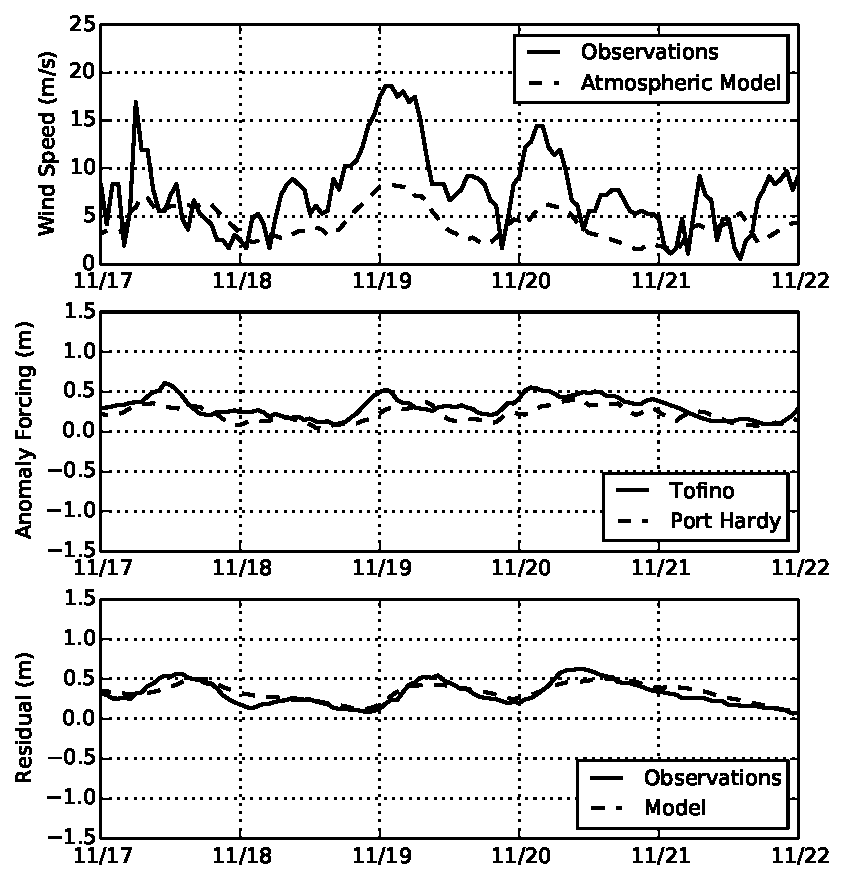
\includegraphics[scale=0.6]{Figures/nov2009.pdf}
\caption{Wind and storm surge conditions at Point Atkinson for a strong wind event on Nov 19, 2009. Top: Wind speed from Environment Canada observations at Point Atkinson (solid) and from the atmospheric model (CGRF) at a grid point near Point Atkinson (dashed). Middle: Sea surface height anomaly at Tofino (solid) and Port Hardy (dashed) used as forcing conditions at the western and northern open boundaries. Bottom: Observed (solid) and modelled (dashed) residuals at Point Atkinson.  }
\label{fig:nov2009}
\end{figure}

%\subsection{High Resolution Atmospheric Forcing: Dec 17, 2012}


\section{Discussion}\label{sec:diss}
%future directions: running real time, biology and chemistry, model improvements?
%comments on wetting and drying (maybe most important in shallow regions)

\section{Appendix}
\begin{table}[h]
\centering 
\begin{tabular}{l l c c c c c c} 
\hline 
& & \multicolumn{3}{c}{M$_2$} & \multicolumn{3}{c}{K$_1$} \\ 
\hline 
Station number & Station name & $R$ & $ \Delta \phi$ (deg) & $D$ (cm) & $R$ & $ \Delta \phi$ (deg) & $D$ (cm) \\
\hline 
               &              &     &                      &          &     &                      &          \\
\hline   
Mean Error     &              &     &                      &          &     &                      &          \\
RMS Error      &              &     &                      &          &     &                      &          \\
\hline  
\end{tabular}
\caption{Comparisons of modelled and observed amplitudes and phases. $R$ is the ratio of modelled to observed amplitude. $\Delta \phi$ is the difference between modelled and observed phase. $D$ is the complex difference. }
\label{tab:comparison} 
\end{table}
%May have to include station numbers and locations on a map? Maybe on the contour map, overlay with stations and green/red dots (hopefully mostly green)
%Should we use the new method of calculating tides?

\section{Acknowledgements}\label{sec:ack}
We would like to thank Michael Foreman, Diane Masson, and Luc Fillion for providing data used in model set up and evaluation. This project is funded by the Marine Environmental Observation Prediction and Response Network (MEOPAR), a Network of Centres of Excellence of Canada.  
%I'm likely missing a lot more (Keith, Youyu, Vasily, JP, Rich, Mark). Not sure about authorship but something to think about for later....

\bibliographystyle{chicago}
\bibliography{ref}

\end{document}

